\section{Suivi d'obstacles}

\subsection{Association d'objets}
\tab À ce stade, notre système est en mesure de nous fournir à un instant t donné / à une itération donnée, une liste d'obstacles qui ont été détectés par le LiDAR sur cette itération. Nous pourrions tout à fait nous en contenter mais l'objectif ici est d'essayer de soutirer un maximum d'informations sur nos obstacles à partir de leur position à cet instant. Concrètement, si nous sommes en mesures de savoir où cet obstacle se trouvait à l'instant précédent, nous pouvons en déduire sa vitesse instantanée. Supposons que l'on arrive à le suivre pendant plusieurs secondes, nous pouvons très bien imaginer une spéculation sur la trajectoire que va suivre l'obstacle et donc anticiper sa position sur l'itération d'après. \\
Notre problème ici est alors dans le fait d'associer les mesures entre deux instants. Comment savoir si l'obstacle X mesuré à l'instant t correspond à l'obstacle Y mesuré à l'instant $t+\Delta t$. Notre démarche a été de prendre la méthode la plus simple possible et d'essayer si cela ne suffisait pas une méthode plus complexe et plus élaborée. \cite{LIDAR2D} \cite{tutoSLAM} \cite{memoire1} \cite{MCMC-SLAM}

\subsubsection{Méthode d'association d'objet}
\tab L'association d'objet est le cœur de notre problème et de notre projet, c'est cette association qui conditionne le bon déroulement de la suite et qui conditionne la véracité de l'analyse des données du LiDAR. Notre algorithme procède donc de la façon suivante:

\begin{enumerate}
    \item Pour chaque obstacle crée à l'itération i-1 :
        \tab \begin{enumerate}
            \item On mesure sa distance par rapport à chaque obstacle créé à l'itération i
            \item On prend le minimum de cette liste de distance
            \item On vérifie que cette distance est inférieure à un seuil défini empiriquement. Ce seuil nous permet d'éviter des vitesses aberrantes si jamais on détecte un unique obstacle d'un côté à l'itération i-1 et un autre unique obstacle complètement à l'opposé à l'itération i.
            \item On considère alors que ces deux obstacles issus de l'itération i-1 et i sont les mêmes et on met alors à jour la position du dit obstacle créé à l'itération i-1.
        \end{enumerate}
    \item Si l'itération i possède plus d'obstacles que l'itération i-1, on aura des obstacles sans association, ce sont donc de nouveaux obstacles que l'on créé. 
    \item À l'inverse, si l'itération i possède moins d'obstacles que l'itération i-1, des obstacles déjà créés vont être dépourvus d'association. Cela signifie que l'obstacle n'a pas été vu à l'itération i donc que l'obstacle n'est plus présent. On détruit alors ces obstacles.
\end{enumerate}
\tab De cette façon, nous sommes en mesure d'actualiser en temps réel la position de nos obstacles.\cite{multi-target-lidar} C'est cette association qui va nous permettre de suivre les obstacles. Notre expérience sur la mise en place d'associations montre que l'utilisation de simples distances entre obstacles fonctionne plutôt bien. Il existe d'autres méthodes qui n'ont pas été développées ici mais qui sont envisageables pour améliorer le système comme l'algorithme de Kuhn-Munkres (aussi appelé algorithme hongrois) qui est un algorithme d'optimisation combinatoire et se prête bien à notre problème. Cet algorithme est notamment utilisé en surveillance pour suivre des personnes sur un flux vidéo.
%peut être parler d'un futur algo hongrois, sinon distance simple comme on l'a fait

\subsection{Détection de murs}
\tab Nous avons déterminé que les objets que nous estimons “d’intérêt” sont en réalité les murs, puisque ce sont des éléments fixes qui permettent de se repérer dans l’espace, et ainsi de les séparer des obstacles mobiles qui seront aussi à éviter. La détection de murs est aussi un élément essentiel d'algorithmes tels que SLAM. Un algorithme de \textit{RANSAC} (pour \textit{RANdom SAmple Consensus}) nous a permis de détecter ces murs afin de les rendre utilisables par d’autres algorithmes dans le cas où la plateforme robotique qui supportera notre LiDAR en aurait besoin.

% expliciter l'algorithme RANSAC en pseudo-langage

Cet algorithme est très efficace pour faire un traitement rapide d'images et obtenir rapidement les éléments linéaires d'un nuage de points, mais il a l'énorme inconvénient de ne pas être déterministe, et dans notre cas on observait qu'environ 1 fois sur 4 l'algorithme ne détectait pas certains murs, ce qui peut être risqué dans une application comme la notre. Nous avons donc décidé de ne pas l'utiliser pour le moment, et de considérer les lignes comme des obstacles comme les autres. De plus, notre objectif n'étant pas un SLAM mais seulement une localisation d'obstacles, cet algorithme n'était en aucun point essentiel.

D'autres algorithmes existent, par exemple ceux utilisant la \textit{transformée de Hough}, permettant de détecter toutes les structures linéaires dans un nuage de point. Cet algorithme, bien que plus lent, serait parfait pour notre application. Une parallélisation sur un Thread à part permettrait de continuer de traiter les données, et périodiquement récupérer les éléments linéaires des nuages de points.

% expliciter l'algorithme de Hough en pseudo-langage

%insérer image RANSAC
\subsection{Filtre de Kalman}
% détailler un peu l'aspect mathématique, ça pourrait être sympa je pense. Du moins de manière très succinte
\tab Une tâche, effectuée en parallèle avec la détection de murs, a été l'implémentation d'un Filtre de Kalman. C'est un algorithme de filtrage de données très populaire car très puissant. Il est utilisé dans toute application requérant un suivi de mesures sur une cible récupérées d'un capteur très bruité.\cite{efk}
Il comprend deux étapes qui se succèdent à chaque mise à jour des données:
\tab \begin{enumerate}
            \item \textit{Prédiction}: On utilise l'état actuel de l'objet mesuré, si il existe, pour essayer de prédire sa prochaine position réelle. On essaye aussi de prédire la matrice de covariance de l'erreur, un élément essentiel du filtre estimant entre autres la précision de l'état estimé.
            \item \textit{Mise à jour}: Après réception des nouvelles mesures, pour l'état suivant, on met à jour l'estimation de l'état de l'objet, c'est à dire son vecteur (position, vitesse), ainsi que l'estimation de sa matrice de covariance de l'erreur.
        \end{enumerate}
        
L'enchaînement de ces deux étapes permettent un suivi très peu bruité de la trajectoire des obstacles suivis. Sur l'image ci-dessous, la position mesurée est en orange, la position obtenue avec le filtre de Kalman est représentée en rouge, et les positions précédentes du centre de l'objet sont représentées en noir, ce qui constitue la \textit{piste}. En cas d'affichage de la position mesurée seulement, on verrait des trajectoires erratiques, en zig-zags de plusieurs cm de large. Ici, nous avons des courbes quasiment lisses, proches des trajectoires réelles des objets.

L'un des inconvénients au filtre de Kalman est qu'il ajoute des petits délais de réaction aux mouvements des cibles. Mais en calibrant bien le filtre nous sommes parvenus à minimiser ces délais tout en gardant des trajectoires bien fluides. Dans le cas du filtre de Kalman simple seuls sont modifiables 3 paramètres: l'écart type du processus, les écarts-types des mesures sur chaque axe, pour lesquels les valeurs empiriques optimales sont dans notre cas respectivement 15, 35mm et 35mm.
%\begin{figure}[htp]
%    \centering
%    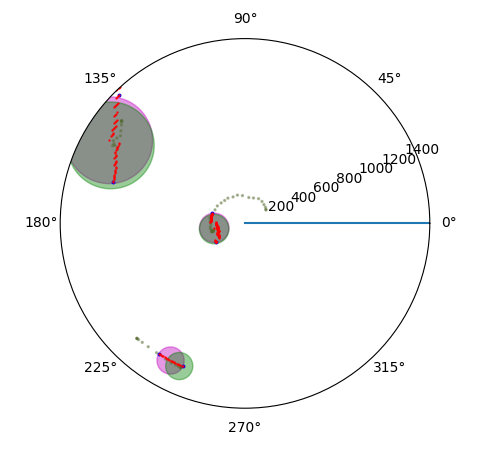
\includegraphics[width=10cm]{images/Suivi/piste01.png}
%    \caption{Piste des objets avec l'affichage polaire.}
%\end{figure}
\begin{figure}[htp]
    \centering
    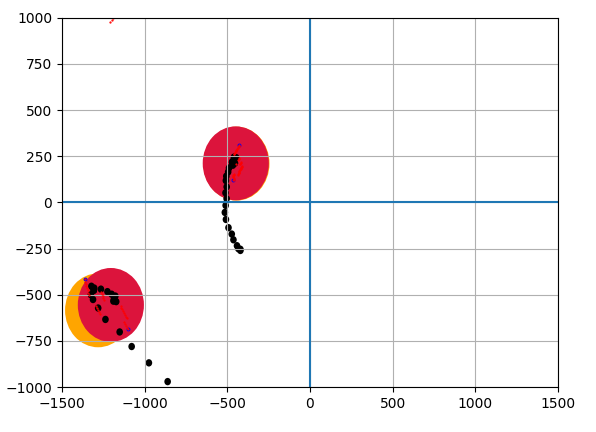
\includegraphics[width=14cm]{images/Suivi/piste02.png}
    \caption{Piste des objets avec l'affichage  cartésien.}
\end{figure}